\chapter{世界面、ウィック回転、チャネル双対性}

\lectureoverview{粒子は世界線を描き、弦は世界面を掃き出す。どちらを量子化するにも経路の和が必要だが、ローレンツ的な和は振動的で定義が難しい。世界面の時間を虚数座標に変えると、ラプラス方程式に支配されるユークリッド理論が得られる。その共形対称性により、4本の弦の相互作用のスリット面は4つの境界挿入を持つ円板となり、直接チャネルと交差チャネルの間の対称性が見えるようになる。}

\section{世界線から経路の和へ}

自由粒子から始める。非相対論的力学ではその位置は関数\(\mathbf x(t)\)であり、質量を一に設定すると、その作用は
\begin{equation}
  S_{\mathrm{NR}}[\mathbf x]
  =\frac12\int_{t_1}^{t_2}\dot{\mathbf x}^{\,2}\,dt.
  \label{eq:l07-nr-action}
\end{equation}
である。相対論的記述では、時間と空間を一つのベクトル\(X^\mu(\tau)\)にまとめ、軌道に沿って\(\tau\)でパラメータ付けする方が自然である。対応する二次式は
\begin{equation}
  S_{\mathrm{rel}}[X]
  =\frac12\int_{\tau_1}^{\tau_2}
  \frac{dX^\mu}{d\tau}\frac{dX_\mu}{d\tau}\,d\tau.
  \label{eq:l07-rel-action}
\end{equation}
である。上付き添字と下付き添字は、時間と空間の間のローレンツ的な符号の違いを表している。
\editorialnote{二次の相対論的作用は、固定された世界線パラメータ付けで用いられている。明白に再パラメータ化不変な代替案は固有長に比例するものであり、それについては講義の後半で言及する。}

\begin{figure}[H]
  \centering
  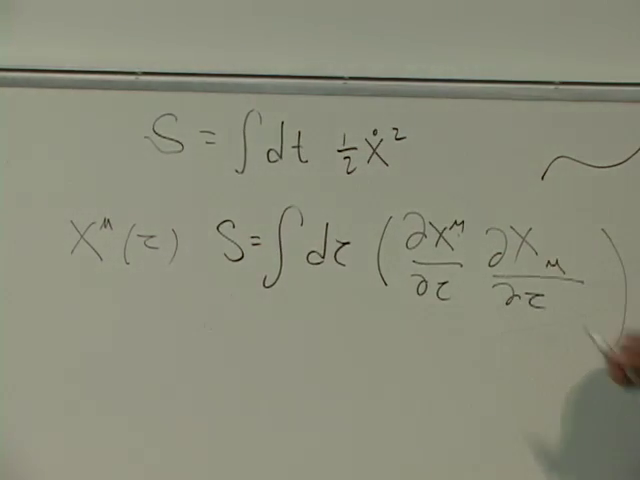
\includegraphics[width=0.72\textwidth]{lecture_07_figure_01.png}
  \caption{非相対論的作用とその相対論的二次対応物を黒板に並べて書いたもの。}
  \lectureframe{00:03:35}
  \label{fig:l07-particle-actions}
\end{figure}

古典的には、端点を固定して経路を変分する。すると自由粒子は一定の速度でまっすぐな世界線をたどる。量子力学は別の問いを立てる。それは端点間の1つの軌道を選び出すのではなく、一方の点で始まり他方の点で検出される確率振幅を問う。その間のあらゆる経路が位相
\begin{equation}
  K(2,1)=\int_{X(1)}^{X(2)}\!\mathcal D X\,
  e^{iS[X]}.
  \label{eq:l07-feynman-integral}
\end{equation}
を寄与する。経路積分は無限次元の経路空間にわたる積分であり、作用の中にすでに現れている通常の積分ではない。

\begin{figure}[H]
  \centering
  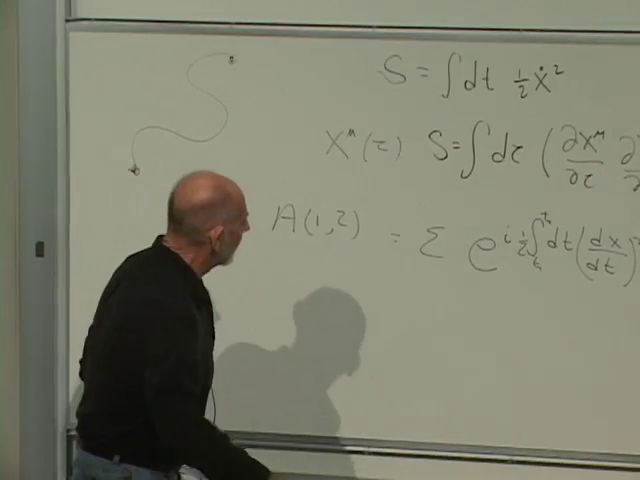
\includegraphics[width=0.72\textwidth]{lecture_07_figure_02.png}
  \caption{代表的な経路と、すべての軌道にわたる和を取る前にそれに割り当てられる位相。}
  \lectureframe{00:06:21}
  \label{fig:l07-path-integral-board}
\end{figure}

相対論的言葉では、この点から点への振幅は伝播関数である。相互作用では、いくつかの世界線の断片が出会う。それらの作用が加えられ、出会いの点について積分され、必要な外部粒子を持つ図が足し合わされる。したがって、おなじみのファインマン図展開は、経路の和を取れという指示の中にすでに暗黙に含まれている。

記号\(S\)はここでは作用を表す。それはエントロピーとも、講義の終わり近くで用いられるマンデルスタム変数\(s\)とも無関係である。この記法の共有は、啓発的というより伝統的なものである。

\section{時間を横に倒す}

\eqref{eq:l07-feynman-integral}には直ちに問題がある。すべての因子\(e^{iS}\)は大きさが1である。したがって、激しく振動する軌道と古典的な直線は等しい絶対的重みで入り、異なるのは位相だけである。破壊的干渉が古典的振る舞いを回復するが、それは形式的な積分を通常の収束する対象にするものではない。

新しいパラメータ\(s\)を
\begin{equation}
  \tau=\alpha s,
  \qquad
  d\tau=\alpha\,ds,
  \qquad
  \frac{dX}{d\tau}=\frac{1}{\alpha}\frac{dX}{ds}.
\end{equation}
によって導入する。すると二次作用は
\begin{equation}
  \frac12\int d\tau
  \left(\frac{dX}{d\tau}\right)^2
  =
  \frac{1}{2\alpha}\int ds
  \left(\frac{dX}{ds}\right)^2.
  \label{eq:l07-rescaled-action}
\end{equation}
と再スケールされる。\(\alpha=-i\)に対応する積分路を選ぶと、振動的な重みは
\begin{equation}
  e^{iS}
  \longrightarrow
  \exp\!\left[-\frac12\int ds
  \left(\frac{dX}{ds}\right)^2\right]
  =e^{-S_E}.
  \label{eq:l07-euclidean-particle}
\end{equation}
に変わる。

\begin{figure}[H]
  \centering
  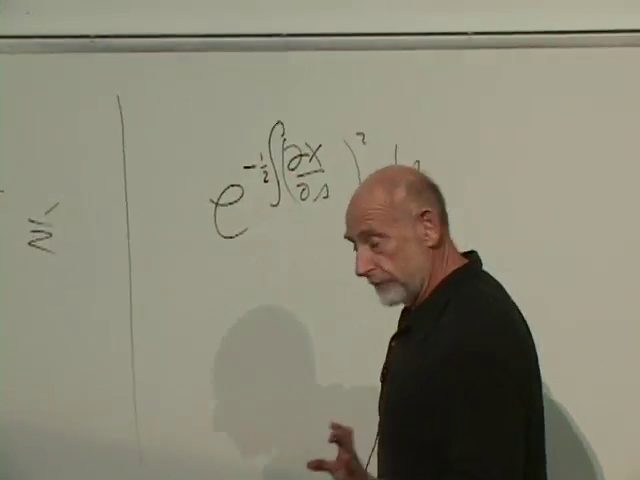
\includegraphics[width=0.66\textwidth]{lecture_07_figure_03.png}
  \caption{虚時間への置き換え後のユークリッド的粒子の重み。指数は実で非正である。}
  \lectureframe{00:16:20}
  \label{fig:l07-particle-wick}
\end{figure}

遠くまで行って戻る経路や、遠くへ行かずに速く揺れる経路は、大きな正の\(S_E\)を持ち、指数的に抑制される。結果はウィーナー型の積分であり、それには厳密な収束理論が存在する。実の\(\tau\)から受け継がれた端点は、虚の\(s\)輪郭上にある。実際には、ユークリッド的対象をその収束領域で評価し、その答えを物理的なローレンツ的変数へ解析接続して戻す。この操作がウィック回転である。時間は計算のために横に倒されたのであって、捨て去られたのではない。

\section{世界線から世界面へ}

点粒子は世界線を持つ。開弦はリボンを掃き出し、閉弦は管を掃き出す。座標\((\sigma,\tau)\)はこの2次元世界面上の点をラベル付けし、
\begin{equation}
  X^\mu=X^\mu(\sigma,\tau)
  \label{eq:l07-embedding}
\end{equation}
はラベル付けされた点の時空位置を与える。すべての関数\(X^\mu\)を知ることは、弦の完全な履歴を指定することである。

二次のローレンツ的ワールドシート作用は、通常の振動する弦と同じく運動エネルギーからポテンシャルを引いた構造を持つ：
\begin{equation}
  S_{\mathrm{ws}}[X]
  =\frac{T_s}{2}\int d\tau\,d\sigma\,
  \left[
    \partial_\tau X^\mu\partial_\tau X_\mu
    -
    \partial_\sigma X^\mu\partial_\sigma X_\mu
  \right].
  \label{eq:l07-lorentzian-worldsheet}
\end{equation}
全体の張力\(T_s\)がスケールを定める。講義ではこれを抑え、微分構造に集中する。

\begin{figure}[H]
  \centering
  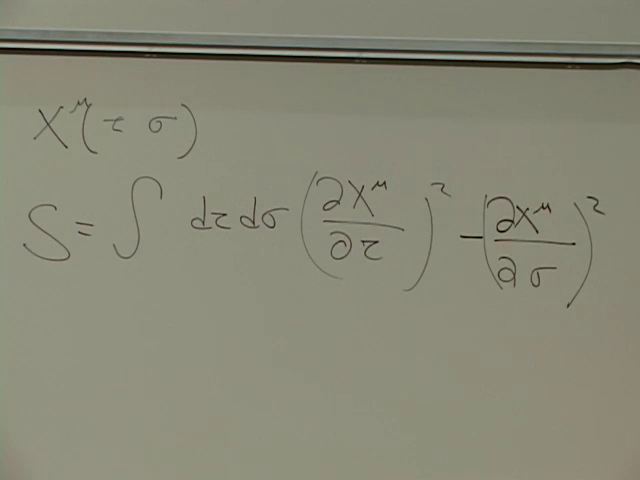
\includegraphics[width=0.72\textwidth]{lecture_07_figure_04.png}
  \caption{\(X^\mu(\sigma,\tau)\)に対するローレンツ的ワールドシート作用。運動エネルギーからポテンシャルを引く符号を持つ。}
  \lectureframe{00:24:26}
  \label{fig:l07-worldsheet-action}
\end{figure}

弦の振幅は、この作用を指数化し、指定された初期と最終の弦配置をつなぐすべての曲面について和を取ることで得られる：
\begin{equation}
  \mathcal A=\int\mathcal D X\,e^{iS_{\mathrm{ws}}[X]}.
  \label{eq:l07-surface-integral}
\end{equation}
同じ規則が、二本の弦が二本になる場合、二本が三本になる場合、その他の許される外部配置を扱う。異なるワールドシートのトポロジーも和に含まれる。穴を加えることは、点粒子の図の展開でループ次数を加えることの弦における対応物である。

\begin{figure}[H]
  \centering
  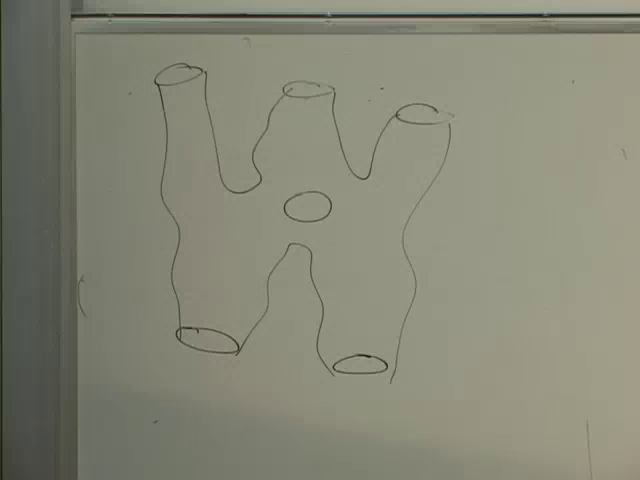
\includegraphics[width=0.66\textwidth]{lecture_07_figure_05.png}
  \caption{複数の外部弦をつなぐ曲面。穴が異なるワールドシートのトポロジーを表す。}
  \lectureframe{00:27:14}
  \label{fig:l07-surface-topology}
\end{figure}

\begin{classroomqa}
\audiencequestion{点状の電子に対して、\(\sigma\)微分は単に消えるのか。\lecturetimestamp{00:27:56}}
\lecturerresponse{点粒子にはそもそも\(\sigma\)座標が存在しない。それでも両者の描像はつながっている。外部状態が弦のスケールに比べて軽く、過程のエネルギーが低いとき、弦の振幅は通常の点粒子ファインマン図を再現する。その極限は、一つの微分をゼロに設定すること以上のものである。}
\end{classroomqa}

面積分は経路積分と同じ収束の問題を持つ。ワールドシート時間をウィック回転した後、その安定なユークリッド形は
\begin{equation}
  \begin{aligned}
    S_{E,\mathrm{ws}}[X]
    &=\frac{T_s}{2}\int d\tau\,d\sigma\,
      \left[
        \partial_\tau X^\mu\partial_\tau X_\mu
        +\partial_\sigma X^\mu\partial_\sigma X_\mu
      \right],\\
    \mathcal A_E&=\int\mathcal D X\,e^{-S_{E,\mathrm{ws}}}.
  \end{aligned}
  \label{eq:l07-euclidean-worldsheet}
\end{equation}
両方の微分が今や同じ正の符号で入る。激しく振動したり大きく引き伸ばされた曲面は大きなユークリッド作用を持ち、抑制される。

\begin{figure}[H]
  \centering
  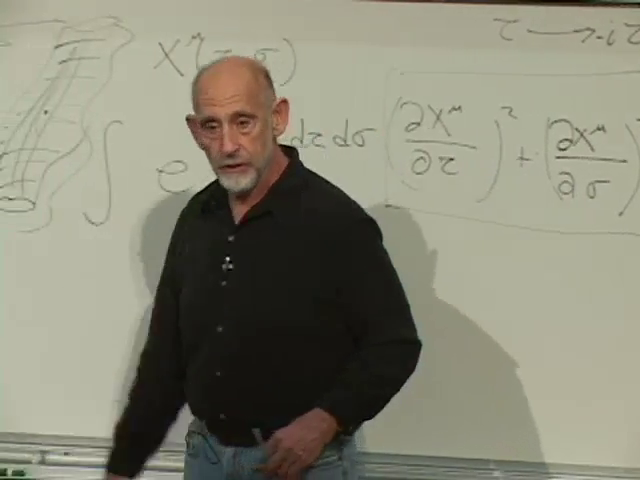
\includegraphics[width=0.72\textwidth]{lecture_07_figure_06.png}
  \caption{\(\tau\)を虚時間に回転した後の正のユークリッド的ワールドシート密度。}
  \lectureframe{00:34:29}
  \label{fig:l07-worldsheet-wick}
\end{figure}

幾何学的に直接的な定式化もある。相対論的粒子にはその経路の固有長に比例する作用を割り当てることができ、弦にはそのワールドシートの時空面積に比例する作用を割り当てることができる。後者が南部--後藤作用である。ここで用いられる二次のワールドシート形式は慣例的にポリアコフ形式と呼ばれ、現在の計算にはるかに容易である。
\editorialnote{講義には歴史的な命名に関するユーモラスな議論も含まれ、関連するリウヴィル作用やディリクレ境界条件にも言及している。導出に優先権の主張は必要ない。面積と補助計量の定式化の等価性のみが用いられる。}

\section{ユークリッド運動方程式}

座標\(\sigma\)と\(\tau\)はシート上のラベルにすぎない。したがって次の問いは避けられない。どのような再ラベル付けが理論を不変に保つのか。その答えは運動方程式から最も容易に見て取れる。\eqref{eq:l07-euclidean-worldsheet}を変分すると、成分ごとに
\begin{equation}
  \partial_\tau^2X^\mu+\partial_\sigma^2X^\mu=0.
  \label{eq:l07-laplace}
\end{equation}
ウィック回転の前は相対符号が負であり、これは波動方程式である。ユークリッド符号では両方の符号が正であるため、二次元ラプラス方程式となる。

\begin{classroomqa}
\audiencequestion{これは振動する太鼓の方程式か。
\lecturetimestamp{00:41:50}}
\lecturerresponse{密接に関係しているが、振動する太鼓は実時間座標も持ち、したがって波動方程式に従う。ここでの方程式はユークリッド的ラプラス方程式である。電荷のない領域における静電ポテンシャルが、より直接的な身近な例を与える。}
\end{classroomqa}

\begin{classroomqa}
\audiencequestion{作用は一階微分を含む。なぜその方程式は二階微分を含むのか。\lecturetimestamp{00:42:44}}
\lecturerresponse{一階微分の二次の項を変分し、部分積分すると、一つの微分がその一階微分の上に移る。これは、作用における\(\dot x^{\,2}\)が運動方程式における\(\ddot x\)を生み出すことの場の理論版である。}
\end{classroomqa}

\begin{figure}[H]
  \centering
  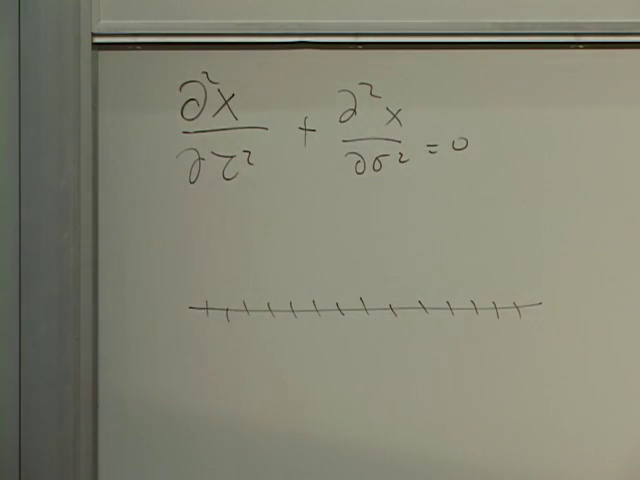
\includegraphics[width=0.68\textwidth]{lecture_07_figure_07.png}
  \caption{正符号のラプラス方程式と、その二階微分を解釈するために用いられた最初の離散的な行。}
  \lectureframe{00:43:30}
  \label{fig:l07-laplace-board}
\end{figure}

幾何学を見るために、まず一つの座標を間隔\(\epsilon\)で離散化する。一階微分は隣接する差であり、二階微分は隣接する差の差である：
\begin{equation}
  \frac{d^2X}{ds^2}\bigg|_{2}
  \longrightarrow
  \frac{X(3)-2X(2)+X(1)}{\epsilon^2}.
  \label{eq:l07-second-difference}
\end{equation}

\begin{figure}[H]
  \centering
  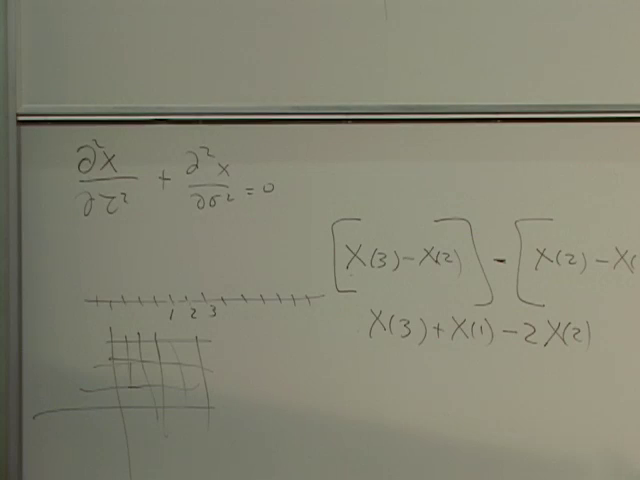
\includegraphics[width=0.72\textwidth]{lecture_07_figure_08.png}
  \caption{番号付きの行、小さな格子パッチ、および二階微分の有限差分展開。}
  \lectureframe{00:45:51}
  \label{fig:l07-finite-difference-board}
\end{figure}

次に\((\sigma,\tau)\)平面を離散化する。中心点\(5\)の四つの最近接点を\(1,2,3,4\)でラベル付けする。式\eqref{eq:l07-laplace}は
\begin{equation}
  X(1)+X(2)+X(3)+X(4)-4X(5)=0,
\end{equation}
または
\begin{equation}
  X(5)=\frac14\bigl[X(1)+X(2)+X(3)+X(4)\bigr].
  \label{eq:l07-mean-value}
\end{equation}

\begin{figure}[H]
  \centering
  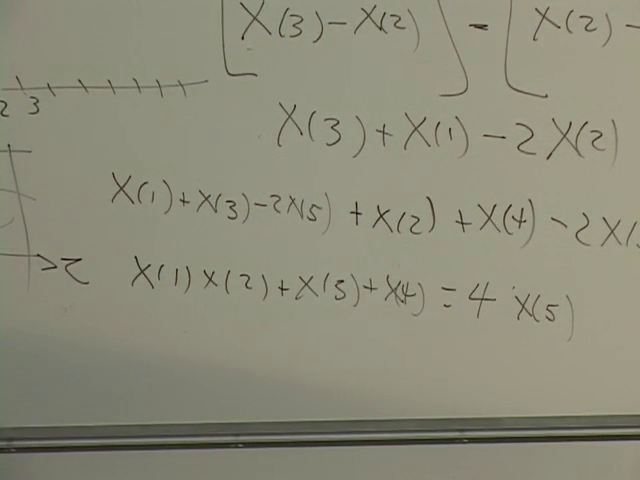
\includegraphics[width=0.72\textwidth]{lecture_07_figure_09.png}
  \caption{完成した二次元有限差分方程式：中心の値は四つの隣接点の平均に等しい。}
  \lectureframe{00:48:26}
  \label{fig:l07-mean-value-board}
\end{figure}

この平均値性質は、任意の向きの無限小正方形に対して成り立つ。これはラプラス方程式の局所的な幾何学的内容であり、共形対称性への橋渡しである。

\section{共形座標}

\((\sigma,\tau)\)から\((\sigma',\tau')\)への変更を考える。一般的な変形は小さな正方形を任意の四辺形に写す。ここで関係する特別な変換は、すべての無限小正方形を、回転およびスケール変更されているかもしれない別の無限小正方形に写す。等価に、それらは曲線の交わる角度を保つ。これらが共形変換である。

\begin{figure}[H]
  \centering
  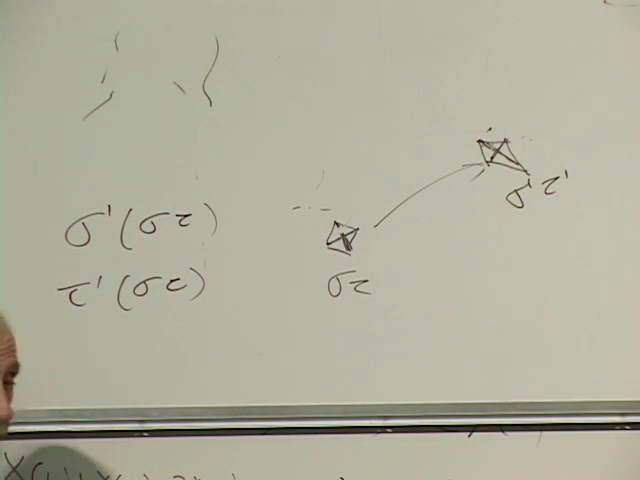
\includegraphics[width=0.68\textwidth]{lecture_07_figure_10.png}
  \caption{局所的な正方形が別の小さな図形に写され、その角度が共形性の保存について調べられている。}
  \lectureframe{00:53:25}
  \label{fig:l07-conformal-board}
\end{figure}

\begin{classroomqa}
\audiencequestion{角度が保たれるなら、変換は基本的に回転だけなのか。\lecturetimestamp{00:53:31}}
\lecturerresponse{局所的にのみであり、しかもそこでも共通のスケール変更も許される。局所的な回転とスケール因子は点ごとに変化しうるので、座標格子は曲がり、ある領域では膨張し、別の領域では収縮しながら、無限小の形を保つことができる。}
\end{classroomqa}

角度を保つ写像は大きさを保つ必要はない。もし大きさも至る所で固定されるなら、可能性ははるかに小さな剛体のクラスである平行移動と回転に縮退してしまう。代わりに共形写像は局所的な形を保つ。これが、地図投影が小さな島の形を保ちながらその面積を大きく歪めうる理由である。

\begin{classroomqa}
\audiencequestion{共形写像は座標系が平坦であることと等価なのか。\lecturetimestamp{00:55:35}}
\lecturerresponse{いいえ。平坦性と共形性は異なる主張である。共形写像は曲がった座標線を用いてもよい。それが保つのは交差する曲線の間の角度である。メルカトル型の地図投影は、大きなスケール歪みを伴う局所的な形の保存の身近な例である。}
\end{classroomqa}

二次元では、必要な変換は複素座標の解析関数によって局所的に生成される
\begin{equation}
  z=\sigma+i\tau.
\end{equation}
有限の境界は見かけを劇的に変えうる。正方形の領域は滑らかな領域に写され、元の角は新しい境界上の目立つ点ではなく、その上の普通の点に送られる。矛盾はない。共形性は局所的な内部の条件であり、写像は正則である至る所で無限小の角度を保つ。

\begin{classroomqa}
\audiencequestion{この座標の自由度が、先ほどの結合--分裂図を対称的に選べた理由なのか。\lecturetimestamp{00:56:32}}
\lecturerresponse{はい。世界面の方程式を保つ同じ共形の自由度によって、扱いにくい相互作用の帯をより対称的な領域に置き換えることができる。残る自由度は物理的な結合--分裂パラメータを除去するのではなく、そのパラメータを境界挿入の相対位置として再包装する。}
\end{classroomqa}

\section{スリットシートと円板}

四本の弦の散乱に戻る。二本の開弦が入射し、それらの端点が結合し、結合した弦が伝播し、後に分裂する。平坦な世界面として描くと、この過程は両端から切り込まれた無限の帯である。スリットの先端の間の間隔\(\tau_0\)は中間弦の寿命であり、振幅はそれについて積分する。

\begin{figure}[H]
  \centering
  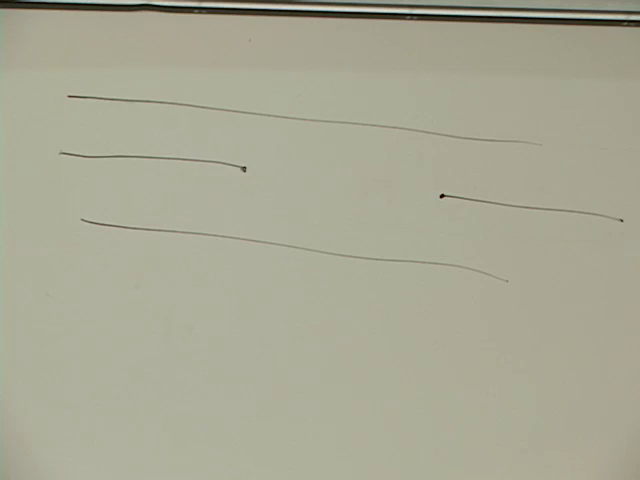
\includegraphics[width=0.72\textwidth]{lecture_07_figure_11.png}
  \caption{二本の開弦が結合し、一緒に伝播し、再び分裂することを表す二重スリット帯。}
  \lectureframe{01:00:20}
  \label{fig:l07-slit-strip}
\end{figure}

ユークリッド化の後、この領域上の埋め込み場はラプラス方程式を満たす。したがって共形不変性により、スリット帯を円板に写すことができる。位相を見る一つの方法は、円板を同心円で葉層化し、それらの閉曲線を連続的に変形してスリット領域を埋め尽くすまでにするものである。無限遠の端は、写像の下で例外的な境界点になる。

\begin{figure}[H]
  \centering
  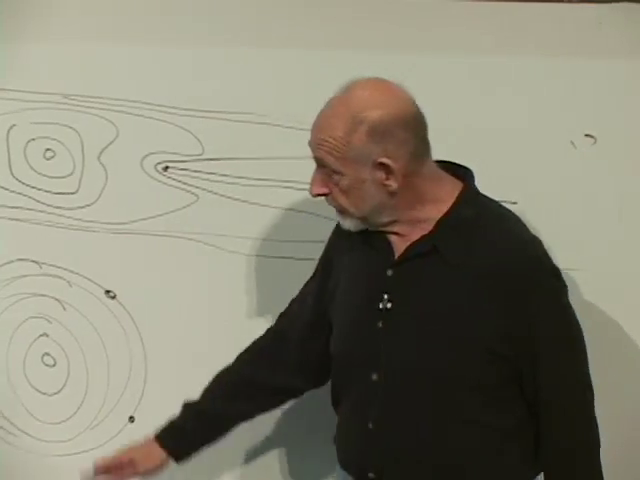
\includegraphics[width=0.72\textwidth]{lecture_07_figure_12.png}
  \medskip

  \begin{adjustbox}{max width=\linewidth}
  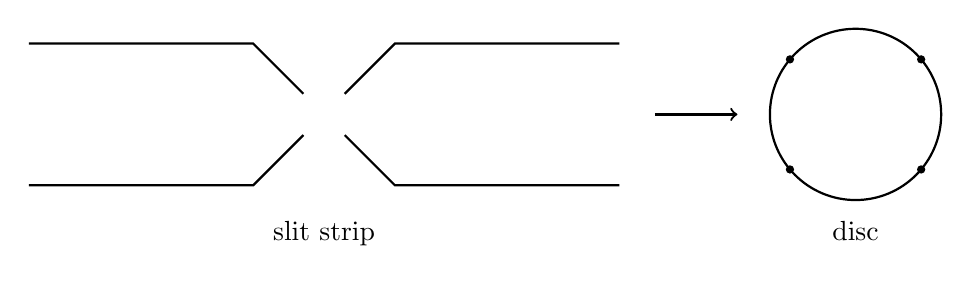
\begin{tikzpicture}[x=0.75cm,y=0.75cm]
    \draw[thick] (-5,1.2) -- (-1.2,1.2) -- (-0.35,0.35);
    \draw[thick] (-5,-1.2) -- (-1.2,-1.2) -- (-0.35,-0.35);
    \draw[thick] (0.35,0.35) -- (1.2,1.2) -- (5,1.2);
    \draw[thick] (0.35,-0.35) -- (1.2,-1.2) -- (5,-1.2);
    \draw[->,thick] (5.6,0) -- (7.0,0);
    \draw[thick] (9.0,0) circle (1.45);
    \foreach \a in {40,140,220,320} \fill (9.0,0) ++(\a:1.45) circle (1.5pt);
    \node[below] at (0,-1.65) {slit strip};
    \node[below] at (9.0,-1.65) {disc};
  \end{tikzpicture}
  \end{adjustbox}
  \caption{板書の等値線の比較と、スリット帯から円板への共形写像の明快な概略図。四つの外部の端は四つの特別な境界点になる。}
  \lectureframe{01:04:46}
  \label{fig:l07-strip-to-disc}
\end{figure}

外部状態はこの座標の変更で失われない。運動量、粒子の種類、振動子の準位は四つの例外的な点に挿入されなければならない。その情報を担う形式的な対象が頂点演算子である。それらの詳細な構成は後回しにするが、その役割はすでに明らかである。それらは、そうでなければ一様な世界面経路積分を、指定された散乱実験に変える。

円板の共形変換を用いて3つの境界点を都合のよい基準位置へ移した後、実の相対位置が1つ残る。それは4つの順序づけられた境界点の交差比で表すことができる。これはかつての寿命\(\tau_0\)の円板版である。

\begin{figure}[H]
  \centering
  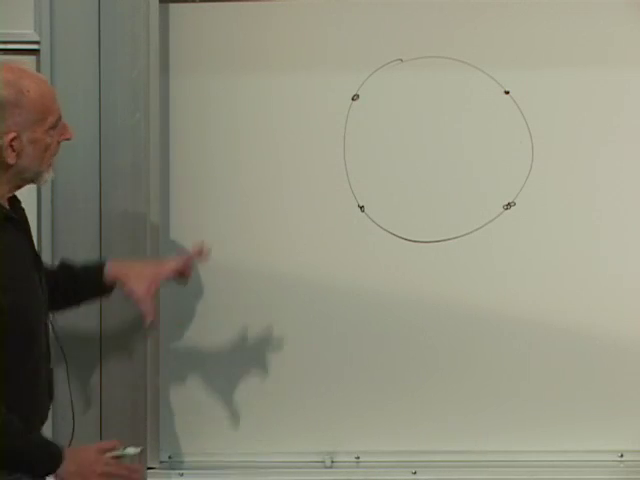
\includegraphics[width=0.62\textwidth]{lecture_07_figure_13.png}
  \caption{円板の境界上の4つの挿入点。共形自由度により、それらの順序づけられた配置の実 modulus は1つを除いてすべて除去される。}
  \lectureframe{01:10:55}
  \label{fig:l07-four-points}
\end{figure}

したがって寿命積分は消えたわけではない。それは残った modulus に関する積分になったのである。従来の座標\(0<z<1\)を用いると、4点開弦積分は前回の講義で得られたのと同じ形をとる。
\begin{equation}
  \mathcal A(s,t)\propto
  \int_0^1 z^{-s-1}(1-z)^{-t-1}\,dz.
  \label{eq:l07-modulus-integral}
\end{equation}

\section{1つの曲面の2つの極限}

moduli 空間の一方の端では、入射対に対応する2つの挿入点が互いに近づく。スリット・ストリップ座標では、これは結合と分裂の間の長い区間である。すなわち直接チャネルの中間弦が長い時間伝播する。もう一方の端では、別の隣接する対が近づく。すると同じ曲面は自然に交差チャネル交換として読まれる。これらの記述はストリップ上では無関係に見えるが、1つの円板積分の隣接する境界極限である。

前回の講義のmostly-plus規約に戻ると、
\begin{equation}
  -s=(k_1+k_2)^2,
  \qquad
  -t=(k_1+k_3)^2.
  \label{eq:l07-mandelstam}
\end{equation}
直接極限は\(s\)における極を整理し、交差極限は\(t\)における極を整理する。
\editorialnote{講義の終わり近くで、黒板ではMandelstam不変量に対して略記号が用いられると同時に、\(s\)が正の重心系エネルギーの二乗であることが同定される。式\eqref{eq:l07-mandelstam}は、講義6で確立されたmostly-plus規約を保っている。}

\begin{figure}[H]
  \centering
  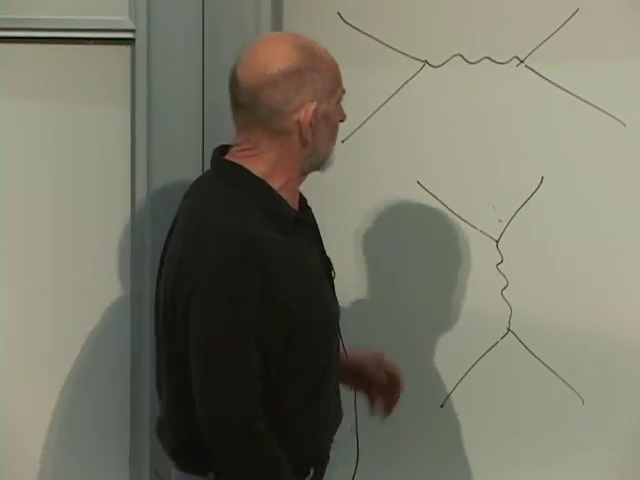
\includegraphics[width=0.62\textwidth]{lecture_07_figure_14.png}
  \caption{2つのチャネル図：一方の向きでの長い伝播と、交差した向きでの交換。}
  \lectureframe{01:19:27}
  \label{fig:l07-channel-diagrams}
\end{figure}

\begin{figure}[H]
  \centering
  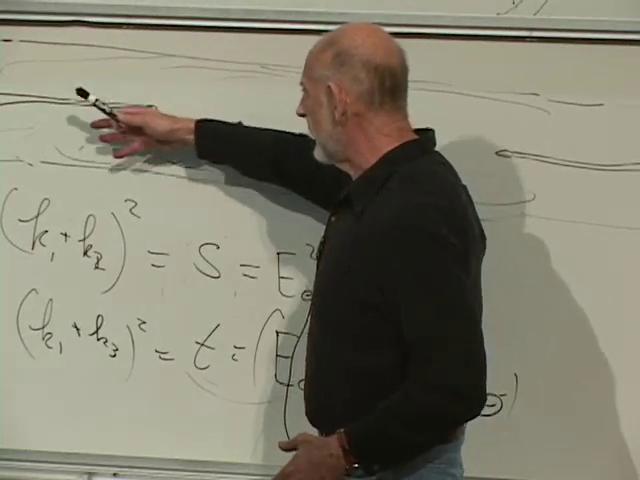
\includegraphics[width=0.72\textwidth]{lecture_07_figure_15.png}
  \caption{黒板は円板 modulus の2つの極限を比較しながら、\(s\)チャネルと\(t\)チャネルの運動量の対に戻る。}
  \lectureframe{01:19:40}
  \label{fig:l07-st-board}
\end{figure}

したがって1つの解析的対象が両方の展開を与える：
\begin{equation}
  \mathcal A(s,t)=\mathcal A(t,s).
\end{equation}
これがチャネル双対性である。元々の共鳴の言葉では、直接チャネル状態の和が交差チャネル交換も符号化できることは奇跡のように思われた。ユークリッド世界面上では、共形対称性が2つの記述が同じ曲面に属する理由を説明する。歴史的には、この解釈は Veneziano 振幅の1969の発見のごく直後に続いた。

\begin{classroomqa}
\audiencequestion{交差した向きに対応するスリット・ストリップ描像もあるか。\lecturetimestamp{01:20:49}}
\lecturerresponse{あるが、時間と呼ばれる方向を別に選ばなければならない。同じユークリッド曲面を、別の外部端の対が遠い過去と未来にあるようにスライスできる。その代替のスライスこそ、1つの世界面が複数のチャネル解釈を許す理由である。}
\end{classroomqa}

\begin{classroomqa}
\audiencequestion{弦が結合したままでいる時間は結合定数によって決まるのか。\lecturetimestamp{01:21:39}}
\lecturerresponse{固定された寿命は選ばれない。寿命は積分変数であり、すべての値が寄与する。結合定数は結合と分裂の重み---等価に言えば崩壊の強さ---を制御し、振幅に乗法的に入る。それは modulus 積分を置き換えるものではない。}
\end{classroomqa}
